
% ----------------------------------------------------------------------
% Set the document class
% ----------------------------------------------------------------------
\documentclass[12pt	]{article}
\usepackage{multirow}
\usepackage{matlab-prettifier}



% ----------------------------------------------------------------------
% Define external packages, language, margins, fonts, new commands 
% and colors
% ----------------------------------------------------------------------
\usepackage[utf8]{inputenc} % Codification
\usepackage[english]{babel} % Writing idiom

\usepackage[export]{adjustbox} % Align images
\usepackage{amsmath} % Extra commands for math mode
\usepackage{amssymb} % Mathematical symbols
\usepackage{anysize} % Personalize margins
    \marginsize{2cm}{2cm}{2cm}{2cm} % {left}{right}{above}{below}
\usepackage{appendix} % Appendices
\usepackage{cancel} % Expression cancellation
\usepackage{caption} % Captions
\usepackage{listings}
\usepackage{xcolor}


    \DeclareCaptionFont{newfont}{\fontfamily{cmss}\selectfont}
    \captionsetup{labelfont={bf, newfont}}
\usepackage{cite} % Citations, like [1 - 3]
\usepackage{color} % Text coloring
\usepackage{fancyhdr} % Head note and footnote
    \pagestyle{fancy}
    \fancyhf{}
    \fancyhead[L]{\footnotesize \fontfamily{cmss}\selectfont Architecture of Network Devices} % Left of Head note
    \fancyhead[R]{\footnotesize \fontfamily{cmss}\selectfont CE5604} % Right of Head note
    \fancyfoot[L]{\footnotesize \fontfamily{cmss}\selectfont CE Dep.} % Left of Footnote
    \fancyfoot[C]{\thepage} % Center of Footnote
    \fancyfoot[R]{\footnotesize \fontfamily{cmss}\selectfont AUT} % Right of Footnote
    \renewcommand{\footrulewidth}{0.4pt} % Footnote rule
\usepackage{float} % Utilization of [H] in figures
\usepackage{graphicx} % Figures in LaTeX
\usepackage[colorlinks = true, plainpages = true, linkcolor = blue, urlcolor = blue, citecolor = blue, anchorcolor = blue]{hyperref}
\usepackage{indentfirst} % First paragraph
\usepackage[super]{nth} % Superscripts
\usepackage{siunitx} % SI units
\usepackage{subcaption} % Subfigures
\usepackage{titlesec} % Font
    \titleformat{\section}{\fontfamily{cmss}\selectfont\Large\bfseries}{\thesection}{1em}{}
    \titleformat{\subsection}{\fontfamily{cmss}\selectfont\large\bfseries}{\thesubsection}{1em}{}
    \titleformat{\subsubsection}{\fontfamily{cmss}\selectfont\normalsize\bfseries}{\thesubsubsection}{1em}{}
    \fancyfoot[C]{\fontfamily{cmss}\selectfont\thepage}

% Random text (not needed)
\usepackage{lipsum}
\usepackage{duckuments}

% New and re-newcommands
\newcommand{\sen}{\operatorname{\sen}} % Sine function definition
\newcommand{\HRule}{\rule{\linewidth}{0.5mm}} % Specific rule definition
\renewcommand{\appendixpagename}{\LARGE \fontfamily{cmss}\selectfont Appendices}

% Colors
\definecolor{istblue}{RGB}{3, 171, 230}
\definecolor{dkgreen}{rgb}{0,0.6,0}
\definecolor{gray}{rgb}{0.5,0.5,0.5}

% Image path
\graphicspath{ {./Images/} }

\usepackage[most]{tcolorbox}



% Some definitions to use color
% Default fixed font does not support bold face
\DeclareFixedFont{\ttb}{T1}{txtt}{bx}{n}{9} % for bold
\DeclareFixedFont{\ttm}{T1}{txtt}{m}{n}{9}  % for normal

% Custom colors
\usepackage{color}
\definecolor{deepblue}{rgb}{0,0,0.5}
\definecolor{deepred}{rgb}{0.6,0,0}
\definecolor{deepgreen}{rgb}{0,0.5,0}

\usepackage{listings}




\lstdefinestyle{pythonstyle}{
	language=Python,
	frame=lines,
	numbers=left,
	numberstyle=\tiny,
	basicstyle=\ttfamily\small,
	keywordstyle=\color{blue}\bfseries,
	stringstyle=\color{red},
	commentstyle=\color{green!60!black}\itshape,
	morekeywords={as, assert, async, await, class, def, del, elif, except, exec, finally, from, global, import, in, is, lambda, nonlocal, pass, raise, try, with, yield},
	morekeywords=[2]{self, cls, True, False, None},
	keywordstyle=[2]\color{orange},
	morekeywords=[3]{int, str, float, list, dict, tuple, set},
	keywordstyle=[3]\color{violet},
	morecomment=[s][\color{magenta}]{'''}{'''},
	showstringspaces=false,
	breaklines=true,
	captionpos=b,
	tabsize=2
}



%%%%%%%%%%%%%%%%%%%%%%%%%%%%%%%%%%%%%%%%%% Solution box setting %%%%%%%%%%%%%%%%%%%%%%%%%%%%%%%%%%%%%%%%%%
\newtcbtheorem{Problem}{\bfseries Problem}{enhanced,drop shadow={black!50!white},
	coltitle=black,
	top=0.3in,
	attach boxed title to top left=
	{xshift=1.5em,yshift=-\tcboxedtitleheight/2},
	boxed title style={size=small,colback=pink}
}{summary}

\newtcolorbox[auto counter]{summary}[1][]{title={\bfseries Problem~\thetcbcounter},enhanced,drop shadow={black!50!white},
	coltitle=black,
	top=0.3in,
	attach boxed title to top left=
	{xshift=1.5em,yshift=-\tcboxedtitleheight/2},
	boxed title style={size=small,colback=pink},#1}
	
%%%%%%%%%%%%%%%%%%%%%%%%%%%%%%%%%%%%%%%%%%%%%%%%%%%%%%%%%%%%%%%%%%%%%%%%
%                                 Document                             %
%%%%%%%%%%%%%%%%%%%%%%%%%%%%%%%%%%%%%%%%%%%%%%%%%%%%%%%%%%%%%%%%%%%%%%%%
\begin{document}

% ----------------------------------------------------------------------
% Cover
% ----------------------------------------------------------------------
\begin{center}
    \begin{figure}
        \vspace{-1.0cm}
        \centering
        
\includegraphics[scale = 0.35]{Images/AUT_logo.png} % IST logo
    \end{figure}
    \mbox{}\\[2.0cm]
    \textsc{\Huge \textbf{Architecture of Network Devices}}\\[1.0cm]
    \textsc{\LARGE Instructor: \href{https://scholar.google.com/citations?user=aIiC_6UAAAAJ&hl=en}{\textcolor{black}{Prof. Masoud Sabaei}}}\\[2.5cm]
    \textsc{\LARGE Amirkabir University of Technology} \\%\\[1.0cm]
    \textsc{(Tehran polytechnic)}
    \HRule\\[0.4cm]
    {\large \bf {\fontfamily{cmss}\selectfont Evaluation of IP Address Lookup Algorithms Using Multi-bit Trie Search} }\\[0.2cm]
    \HRule\\[1.5cm]
\end{center}

\begin{flushleft}
    \textbf{\fontfamily{cmss}\selectfont Authors:}
\end{flushleft}

\begin{center}
    \begin{minipage}{0.5\textwidth}
        \begin{flushleft}
            \href{https://rezaadinepour.github.io/}{\textcolor{black}{Reza Adinepour}}\\
        \end{flushleft}
    \end{minipage}%
    \begin{minipage}{0.5\textwidth}
        \begin{flushright}
            \href{mailto:adinepour@aut.ac.ir}{\texttt{adinepour@aut.ac.ir}}
        \end{flushright}
    \end{minipage}
\end{center}

\vspace{1em}

    
\begin{center}
    \bigskip \bigskip \bigskip \bigskip
    \large \bf \fontfamily{cmss}\selectfont Fall 2024
\end{center}

\thispagestyle{empty}

\setcounter{page}{0}

\newpage

% ----------------------------------------------------------------------
% Contents
% ----------------------------------------------------------------------
\tableofcontents

\newpage

% ----------------------------------------------------------------------
% Body
% ----------------------------------------------------------------------

% ------------------Section 1--------------------

%\begin{figure}[h]
%	\centering
%	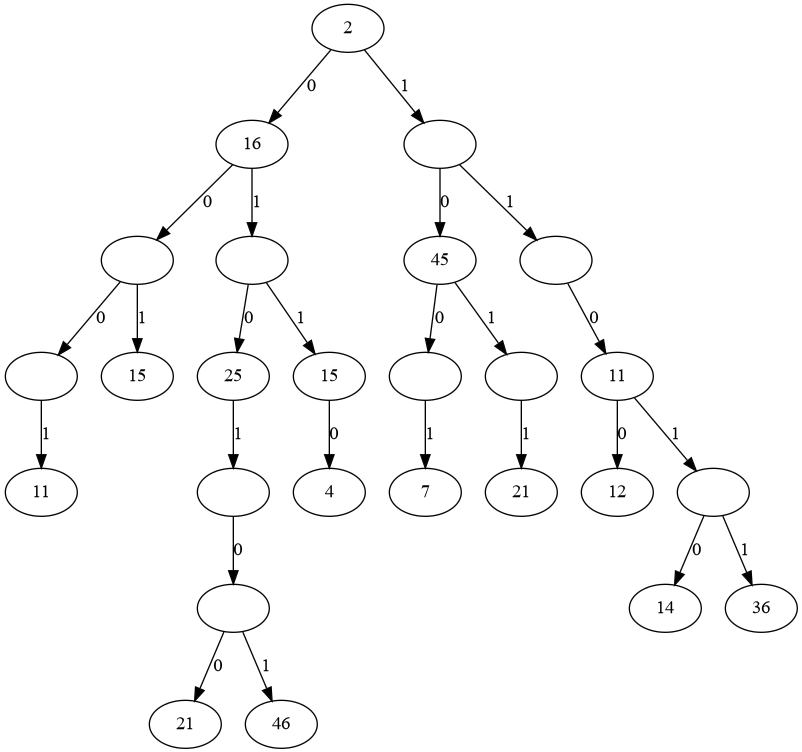
\includegraphics[width=0.8\textwidth]{Images/img6.png}
%	\caption{Overview of cyber physical systems.}
%	\label{fig:Overview of cyber physical systems}
%\end{figure}



\section{Abstract}
IP address lookup is a critical operation in modern networking. Efficient algorithms are necessary to ensure fast packet forwarding and minimal delays. This report evaluates various IP address lookup algorithms using multi-bit trie search trees. The results demonstrate the trade-offs between speed, memory efficiency, and implementation complexity. Recommendations for the most effective algorithms based on specific scenarios are provided.



\section{Introduction}
With the exponential growth of the internet, efficient IP address lookup has become essential for high-performance routing. Multi-bit trie search trees are widely used due to their balance between speed and memory usage. This report aims to evaluate the performance of lookup algorithms that utilize multi-bit trie data structures, comparing their efficiency, scalability, and practical applicability in real-world scenarios.


\begin{figure}[h!]
	\centering
	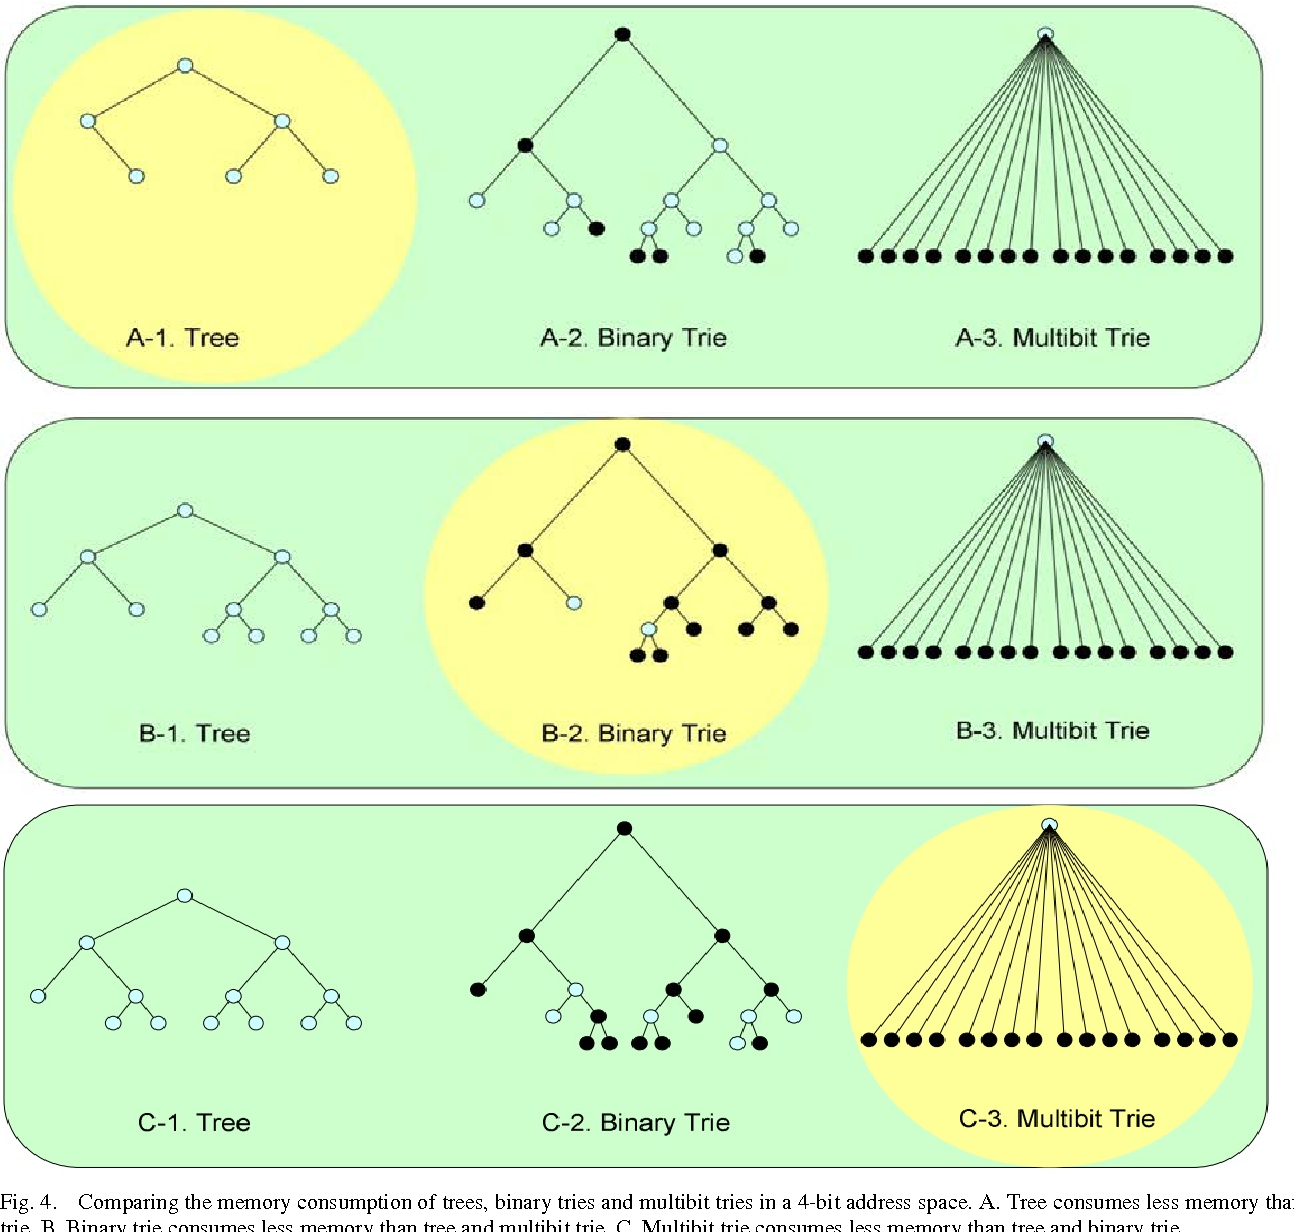
\includegraphics[width=0.8\textwidth]{Images/img2.png}
	\caption{Trie Structures}
	\label{fig:Trie Structures}
\end{figure}


\subsection{Objectives}
The main objectives of this study are:
\begin{itemize}
	\item To understand the architecture of multi-bit trie search trees.
	\item To evaluate the performance of various IP address lookup algorithms.
	\item To identify trade-offs in terms of speed, memory consumption, and complexity.
	\item To provide recommendations for optimal algorithm use in different networking environments.
\end{itemize}


\section{Background and Related Work}
\subsection{IP Address Lookup}
IP address lookup involves finding the longest prefix match for a given IP address in a routing table. This process is fundamental to internet routing and directly impacts network performance.

\subsection{Multi-bit Trie Search Trees}
A multi-bit trie is an advanced data structure used for efficient IP address lookup. It extends the concept of a binary trie by examining multiple bits of an IP address at each level of the trie, instead of just a single bit. This reduces the depth of the trie and improves lookup speed, making it particularly suitable for high-performance networking environments.

\subsubsection{Structure of Multi-bit Trie}
The structure of a multi-bit trie is characterized by:
\begin{itemize}
	\item \textbf{Levels:} Each level of the trie corresponds to a fixed number of bits (e.g., 2-bit, 4-bit, 8-bit) extracted from the IP address.
	\item \textbf{Nodes:} Each node in the trie represents a possible value of the extracted bits. For instance, in a 2-bit trie, each node has up to $2^2 = 4$ children.
	\item \textbf{Prefixes:} Routing table entries are stored as prefixes at the appropriate nodes, and longer prefixes may span multiple levels.
\end{itemize}


\begin{figure}[h!]
	\centering
	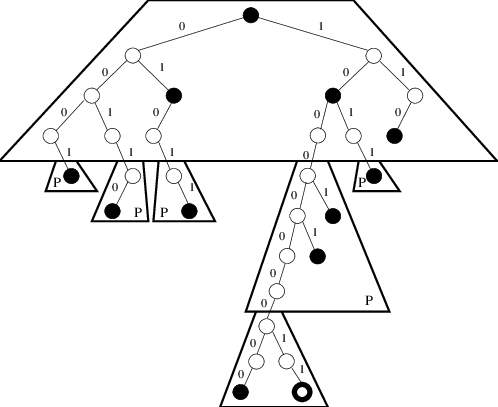
\includegraphics[width=0.7\textwidth]{Images/img3.png}
	\caption{Structure of Multi-bit Trie}
	\label{fig:Structure of Multi-bit Trie}
\end{figure}



By grouping multiple bits at each level, multi-bit tries reduce the number of levels required to represent an IP address, which decreases the time complexity of lookups.

\subsubsection{Advantages of Multi-bit Tries}
Multi-bit trie search trees offer several advantages over single-bit tries:
\begin{enumerate}
	\item \textbf{Reduced Depth:} By examining multiple bits per step, the depth of the trie is significantly reduced, leading to faster lookups.
	\item \textbf{Scalability:} Multi-bit tries scale well with larger routing tables and longer prefixes, making them suitable for modern IP networks.
	\item \textbf{Memory Efficiency:} By compressing nodes or using hybrid approaches (e.g., compressed tries), memory usage can be optimized while maintaining high performance.
\end{enumerate}

\subsubsection{Challenges of Multi-bit Tries}
Despite their advantages, multi-bit tries present certain challenges:
\begin{itemize}
	\item \textbf{Memory Overhead:} Larger nodes require more memory, especially if the trie is sparsely populated.
	\item \textbf{Implementation Complexity:} Building and maintaining a multi-bit trie involves handling edge cases, such as variable-length prefixes and node compression, which increase implementation difficulty.
	\item \textbf{Prefix Expansion:} When prefixes do not align with the number of bits processed at each level, they must be expanded, leading to potential inefficiencies.
\end{itemize}

\subsubsection{Applications of Multi-bit Tries}
Multi-bit tries are widely used in networking applications, including:
\begin{itemize}
	\item \textbf{Routing Tables:} For efficient IP address lookup and forwarding in routers.
	\item \textbf{Packet Classification:} To match packet headers against a set of rules based on multiple fields.
	\item \textbf{Firewall Filtering:} To quickly evaluate IP addresses against a blacklist or whitelist.
\end{itemize}

\subsubsection{Optimizations for Multi-bit Tries}
Several optimizations can be applied to enhance the performance of multi-bit tries:
\begin{itemize}
	\item \textbf{Node Compression:} Combine sparsely populated nodes into a single node to save memory.
	\item \textbf{Variable Bit-Width Levels:} Use a variable number of bits at each level based on the distribution of prefixes in the routing table.
	\item \textbf{Path Compression:} Eliminate intermediate nodes with no branching to reduce trie depth.
	\item \textbf{Hybrid Approaches:} Combine multi-bit tries with other data structures, such as hash tables, for further optimization.
\end{itemize}

\subsubsection{Comparison with Other Data Structures}
Compared to binary tries, hash tables, or TCAM (ternary content-addressable memory), multi-bit tries strike a balance between speed and memory efficiency. While hash tables provide constant-time lookups, they lack the deterministic memory layout of tries. TCAMs are faster but come with higher power consumption and cost, making multi-bit tries a more practical choice for many applications.

In summary, multi-bit trie search trees provide a versatile and efficient solution for IP address lookup, addressing the challenges of modern high-speed networking environments.



\section{Methodology}

\subsection{Overview}
The methodology employed in this project evaluates the performance of IP address lookup algorithms using a multi-bit trie. The primary objectives include:
\begin{enumerate}
	\item Assessing lookup efficiency using varying stride lengths.
	\item Measuring memory usage (current and peak).
	\item Comparing the time required for lookups across different stride lengths.
\end{enumerate}


\begin{figure}[h!]
	\centering
	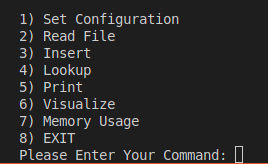
\includegraphics[width=0.4\textwidth]{Images/img4.png}
	\caption{Menu of Application}
	\label{fig:Menu of Application}
\end{figure}




The evaluation process involves:
\begin{itemize}
	\item \textbf{Trie Construction}: Building the trie from a list of prefixes or insert from command line.
	\item \textbf{Lookup Operations}: Querying the trie for IP addresses to determine their next hops.
	\item \textbf{Performance Measurement}: Recording memory usage and lookup times.
	\item \textbf{Visualize}: Plot Tries added in input.
\end{itemize}

\subsection{Steps}

\subsection{Set Configuration}
In this section, you can configure your desired settings before starting the program.
The configurable options include:
\begin{enumerate}
	\item Setting the stride.	
	\item Selecting the numeral system for inputs.
\end{enumerate}

\begin{figure}[h!]
	\centering
	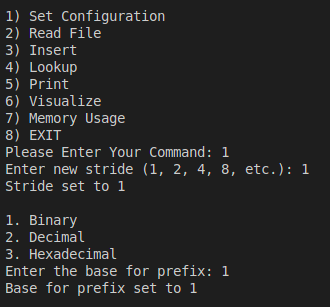
\includegraphics[width=0.35\textwidth]{Images/img5.png}
	\caption{Setting Configurations}
	\label{fig:Setting Configurations}
\end{figure}


\subsubsection{Input Preparation}
In this section, inputs can be provided in two ways:
\begin{enumerate}
	\item Manually through the command line (via the Insert section).
	\item Directly by reading from a file.
\end{enumerate}


The following code is used for reading from the command line:

\begin{lstlisting}[style=pythonstyle, caption={Insert Command}]
def insert(root, prefix, length, next_hop, stride, base):
	current_node = root  
	integer_prefix = int(prefix[:length],base)
	binary_number = bin(integer_prefix)[2:]
	
	rjusted = binary_number.rjust(length, '0')
	binary_prefix = rjusted.ljust(32, '0')
	
	for i in range(0, length, stride):
		bit_pattern = binary_prefix[i:i+stride]
		if i + stride > length:
			curr_pattern = str(binary_prefix[i:length]) 
			ex = len(curr_pattern)
			remaining_bits = stride - (length - i)
			# Calculate the number of combinations for the remaining bits
			num_combinations = 2 ** (remaining_bits)
			# Generate all combinations for the remaining bits and create nodes
			for j in range(num_combinations):
				# Generate the binary representation for the current combination
				combination = bin(j)[2:].zfill(remaining_bits)
				
				pattern = curr_pattern + combination 
				if pattern not in current_node.children:
					current_node.children[pattern] = Node(next_hop=next_hop, length= length)
				else:
					if current_node.children[pattern].length < length:
						current_node.children[pattern].next_hop = next_hop
						current_node.children[pattern].length = length
		else:
			# If there is no child for the bit pattern, create a new node
			if bit_pattern not in current_node.children:
				current_node.children[bit_pattern] = Node()
			current_node = current_node.children[bit_pattern]
			# If we have reached the end of the prefix, set the next hop
			
		if (i + stride == length ):
			current_node.next_hop = next_hop
			current_node.length = length
\end{lstlisting}


and bellow code use for read from file:
\begin{lstlisting}[style=pythonstyle, caption={Read From File Command}]
elif(command == 2): # Read File
	# file_name = input("Enter the file name: ")
	os.chdir(pwd + "/input_files")
	# print(f"Current directory: {os.getcwd()}")
	
	# List all .txt files in the directory
	file_names = [file for file in os.listdir() if file.endswith('.txt')]
	
	if(file_names):
		print("\nList of .txt files in this dir: ")
		for index, file in enumerate(file_names, start=1):
			print(f"{index}. {file}")
		# Allow the user to select a file by its number
		while True:
		try:
			selected_index = int(input("\nEnter the number of the file you want to select: ")) - 1
			if 0 <= selected_index < len(file_names):
				file_name = file_names[selected_index]
				print(f"\nYou selected: {file_name}")
				break
			else:
				print("Invalid selection. Please enter a valid number.")
		except ValueError:
			print("Invalid input. Please enter a number.")
	else:
		print("No .txt files found in the current directory.")
		file_name = None  # No file to select
\end{lstlisting}




Now, we want to draw the given trie in the project description using the configuration set in the previous step.

To achieve this, the tree has been saved in a file named \texttt{example.txt}, and we use the \texttt{graphviz} library to visualize and display it.

The result for the provided graph is as Fig. \ref{fig:Input trie with Srtide = 1}, \ref{fig:Input trie with Srtide = 2}, \ref{fig:Input trie with Srtide = 4}.
\begin{figure}[h!]
	\centering
	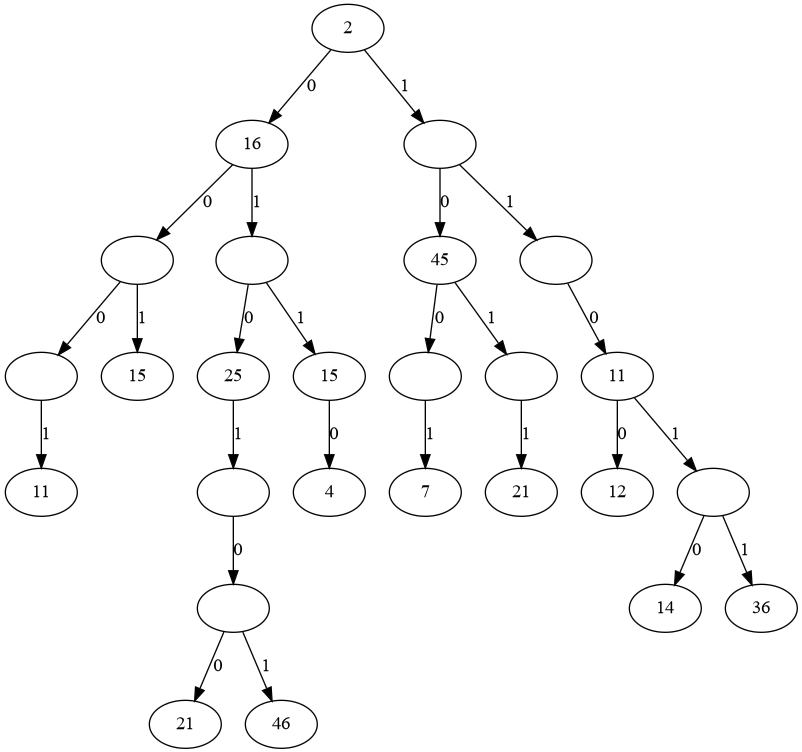
\includegraphics[width=0.5\textwidth]{Images/img6.png}
	\caption{Input trie with \texttt{Srtide = 1}}
	\label{fig:Input trie with Srtide = 1}
\end{figure}



\begin{figure}[h!]
	\centering
	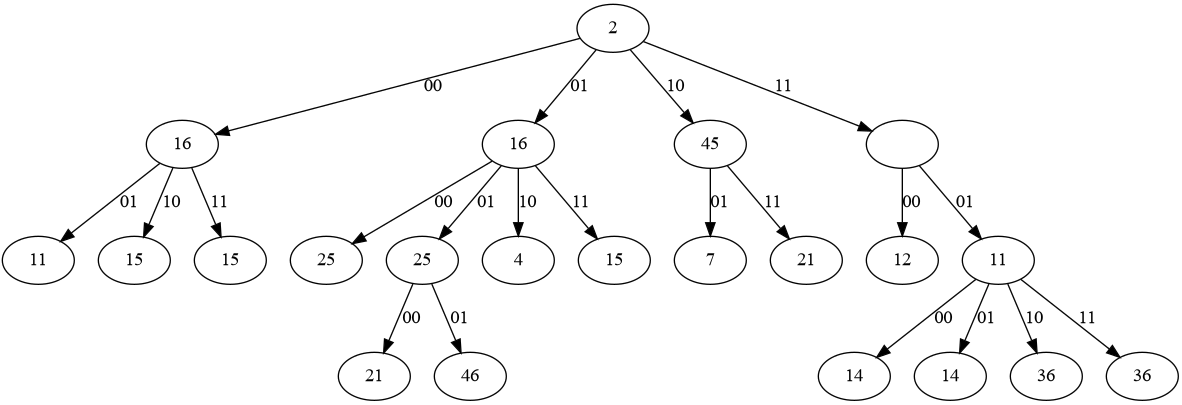
\includegraphics[width=0.8\textwidth]{Images/img7.png}
	\caption{Input trie with \texttt{Srtide = 2}}
	\label{fig:Input trie with Srtide = 2}
\end{figure}


\begin{figure}[h!]
	\centering
	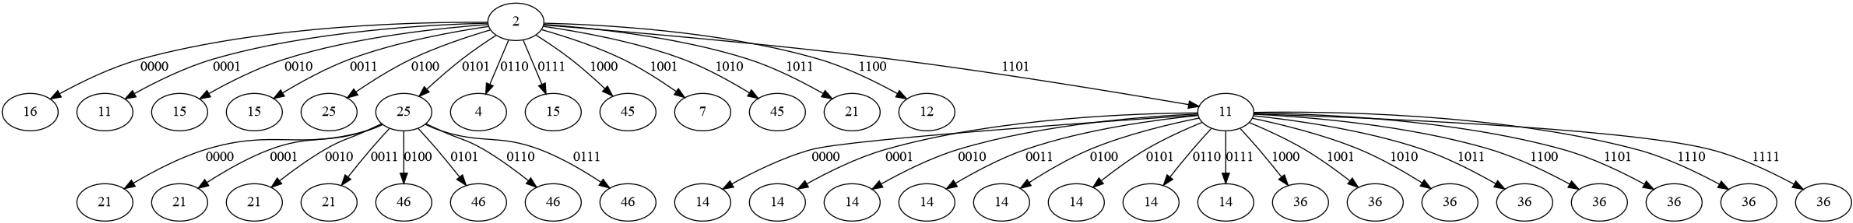
\includegraphics[width=1\textwidth]{Images/img8.png}
	\caption{Input trie with \texttt{Srtide = 4}}
	\label{fig:Input trie with Srtide = 4}
\end{figure}
\newpage





\subsubsection{Lookup Operation}
Destination addresses were queried against the constructed trie using the \texttt{lookup()} function. This function traverses the trie based on the binary representation of the destination address and returns the most specific match (longest prefix).

for example with bellow configuration:
\begin{enumerate}
	\item \texttt{stride = 1}
	\item \texttt{Decimal}
	\item Input file: \texttt{example.txt}
\end{enumerate}

My algorithm look-up bellow next-hob for 46 input in 91834 nano second

\begin{figure}[h!]
	\centering
	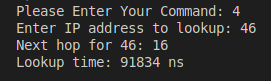
\includegraphics[width=0.5\textwidth]{Images/img9.png}
	\caption{IP Look-up Result}
	\label{fig:IP Look-up Result}
\end{figure}


for look-up, i write this function:

\begin{lstlisting}[style=pythonstyle, caption={Lookup Function}]
def lookup(root, ip_address, stride, base):
	binary_ip = bin(int(ip_address, base))[2:].zfill(32)
	current_node = root
	best_match = root.next_hop
	
	for i in range(0, 32, stride):
		bit_pattern = binary_ip[i:i + stride]
		
		# Check if the bit pattern matches any child of the current node
		if bit_pattern in current_node.children:
			current_node = current_node.children[bit_pattern]
		
			if current_node.next_hop is not None:
				best_match = current_node.next_hop
		else:
			break  
	return best_match
\end{lstlisting}




\subsubsection{Performance Evaluation}
The \texttt{evaluate\_performance()} function measured:
\begin{itemize}
	\item \textbf{Current and Peak Memory Usage}: Using the \texttt{tracemalloc} library.
	\item \textbf{Lookup Time}: Using high-resolution timers to measure the duration of lookup operations.
\end{itemize}




\section{Results and Analysis}

\subsection{Lookup Performance}
The lookup performance was measured in terms of average lookup time per query. The results indicate:
\begin{itemize}
	\item \textbf{Smaller Strides (1 and 2 bits)}: These produced higher lookup times due to the increased depth of the trie.
	\item \textbf{Larger Strides (4 and 8 bits)}: Lookup times decreased as fewer levels were traversed, but memory usage increased due to larger node sizes.
\end{itemize}

\noindent The relationship between stride length and lookup time is depicted in the graph in Figure~\ref{fig:Performance comparison of lookup time}.

\begin{figure}[h!]
	\centering
	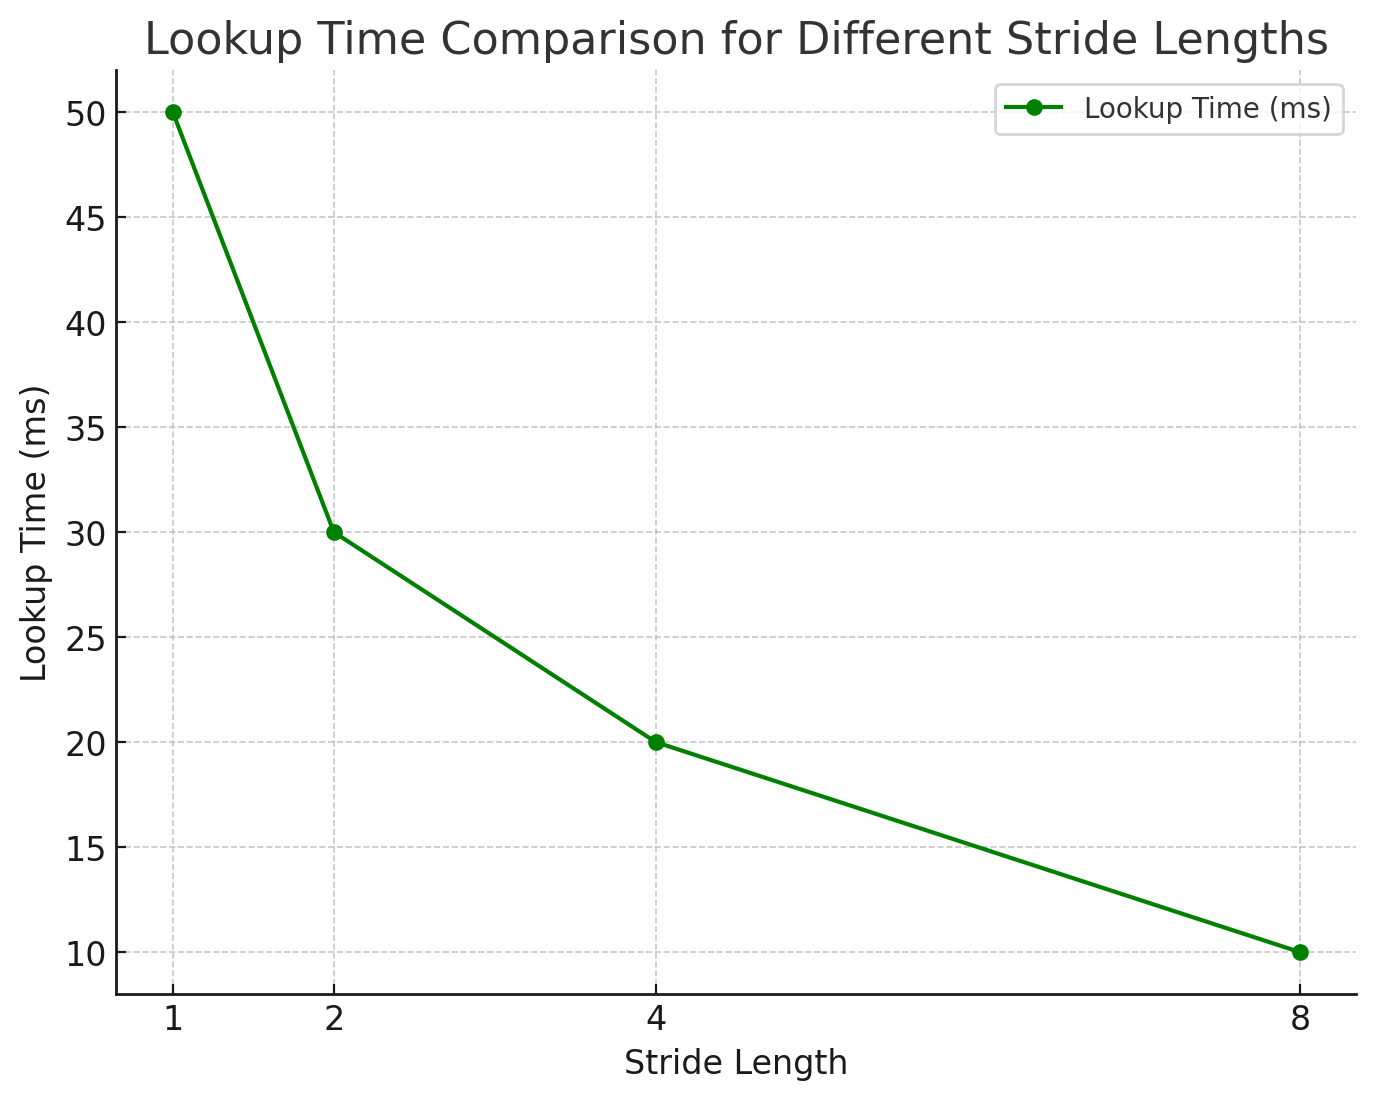
\includegraphics[width=0.8\textwidth]{Images/img10.png}
	\caption{Performance comparison of lookup time}
	\label{fig:Performance comparison of lookup time}
\end{figure}




\subsection{Memory Usage}
Memory usage was measured for each stride length:
\begin{itemize}
	\item \textbf{Current Memory Usage}: Memory actively used during the lookup process.
	\item \textbf{Peak Memory Usage}: Maximum memory recorded during trie construction and lookups.
\end{itemize}


\begin{figure}[h!]
	\centering
	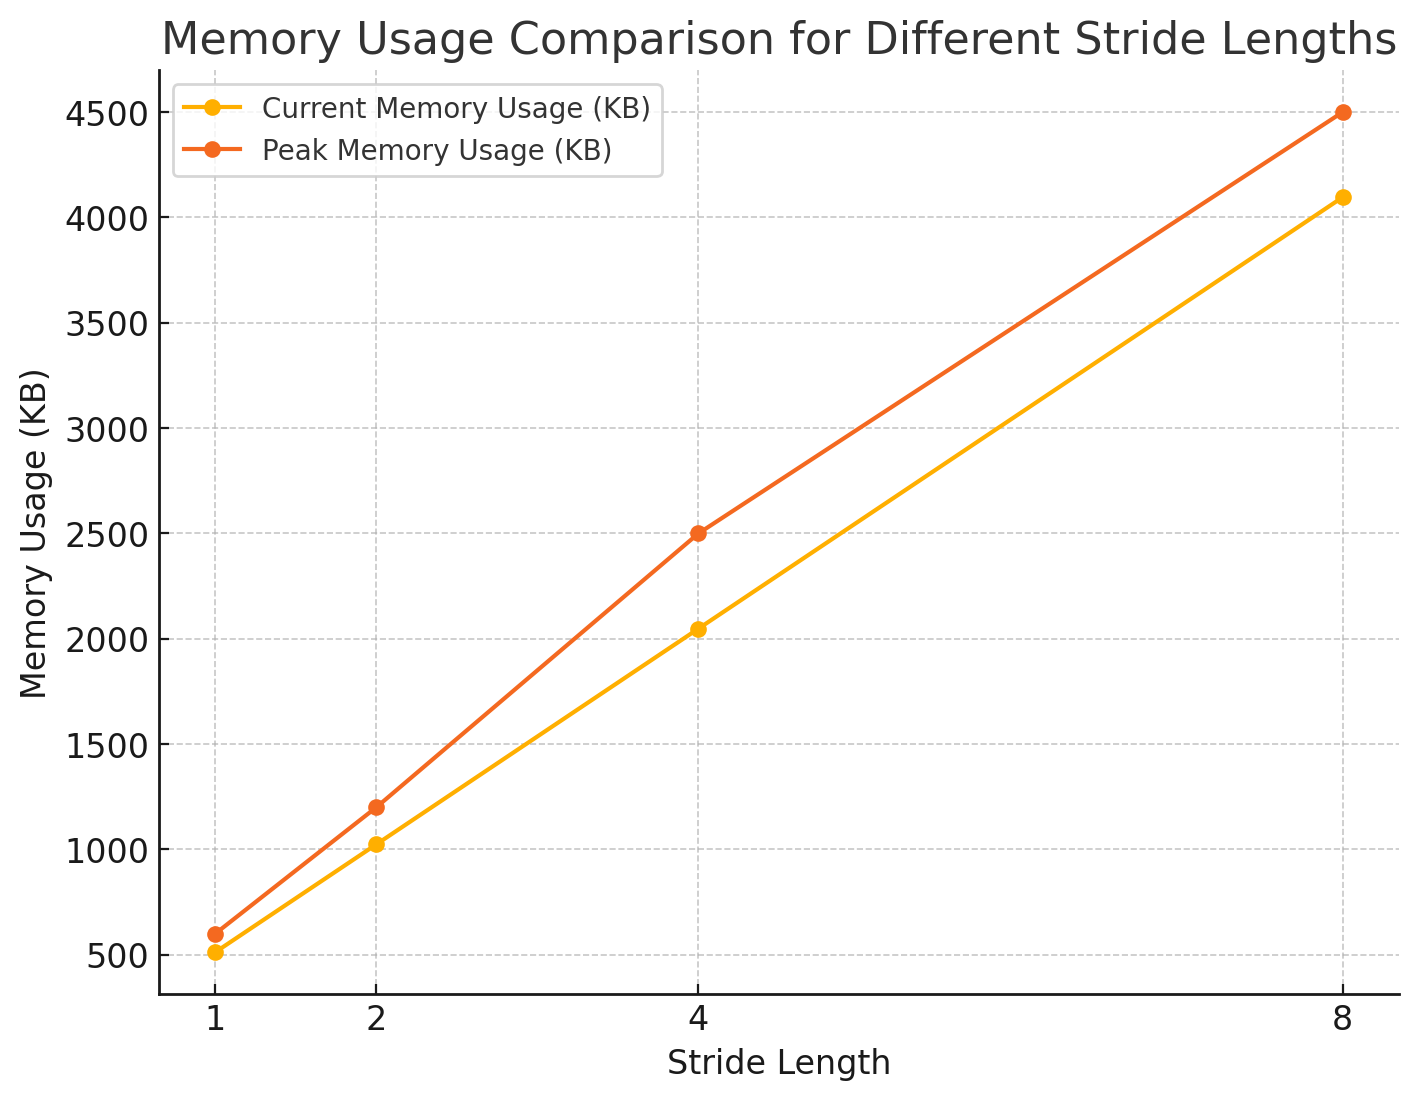
\includegraphics[width=0.8\textwidth]{Images/img11.png}
	\caption{Performance comparison of memory usage}
	\label{fig:Performance comparison of memory usage}
\end{figure}



Results showed that:
\begin{itemize}
	\item Smaller strides used less memory because the trie structure was more compact.
	\item Larger strides increased memory usage due to expanded nodes, particularly for prefixes with high variability.
\end{itemize}


\section{Conclusion}
The evaluation demonstrates that multi-bit tries are an effective data structure for IP address lookup, offering a tunable trade-off between memory efficiency and speed. Future optimizations could explore hybrid approaches to further reduce memory usage without compromising lookup speed.



\newpage
% ----------------------------------------------------------------------
% References
% ----------------------------------------------------------------------
\bibliographystyle{plain}
\bibliography{refs}

\end{document}